\chapter{Circuitos en corriente continua: leyes de Kirchhoff y teoremas}\label{ch:b1:dc-circuits}

Girar la llave en una mañana fría: el motor de arranque gruñe, las luces
del salpicadero se apagan un segundo y el coche arranca entre toses. La
batería que hace un momento entregaba \qty{12.6}{V} constantes ha bajado a
once mientras el motor de arranque consume sus ciento cincuenta \omterm{def:b1:dc-circuits:current}{amperios}
--- y los faros, conectados en paralelo, lo pagan. Todo lo que sucede en
ese segundo lo gobiernan dos leyes de conservación y un puñado de teoremas
sobre \omterm{def:b1:dc-circuits:linear}{circuitos lineales}, que este capítulo enuncia, demuestra y aplica:
las \omterm{thm:b1:dc-circuits:kirchhoff}{leyes de Kirchhoff}, los modelos de fuentes y \omterm{def:b1:dc-circuits:resistor}{resistores}, los
divisores, Thévenin y Norton, y el arte gráfico de hallar un \omterm{met:b1:dc-circuits:loadline}{punto de
funcionamiento}.

\section{Corriente, tensión y régimen cuasiestacionario}

\begin{definition}[Intensidad de corriente]\label{def:b1:dc-circuits:current}
\index{intensidad de corriente}\index{amperio}
La \emph{intensidad de corriente} a través de una superficie (la sección
de un hilo) es la carga que la atraviesa por unidad de tiempo, contada
positivamente en una orientación elegida:
\[
i = \frac{\dd q}{\dd t} \qquad (\text{amperios: } \qty{1}{A} = \qty{1}{C/s}).
\]
Invertir la orientación cambia el signo de $i$. En un metal los portadores
son electrones, que se desplazan \emph{en sentido contrario} al de la
corriente convencional, a una fracción de milímetro por segundo.
\end{definition}

\begin{definition}[Potencial y tensión]\label{def:b1:dc-circuits:voltage}
\index{potencial eléctrico}\index{tensión}\index{masa (referencia)}
Cada punto de un circuito tiene un \emph{potencial eléctrico} $V$
(voltios), definido salvo una constante que se fija eligiendo una
\emph{masa} ($V = 0$). La \emph{tensión} entre $A$ y $B$ es la diferencia
de potencial $u_{AB} = V_A - V_B$, dibujada como una flecha de $B$ hacia
$A$. La energía que pierde una carga $q$ al ir de $A$ a $B$ vale
$q\,u_{AB}$ (esto enlaza con el potencial electrostático de
\cref{ch:b1:potential-capacitors}).
\end{definition}

\begin{definition}[Régimen cuasiestacionario (ARQS)]\label{def:b1:dc-circuits:arqs}
\index{régimen cuasiestacionario}\index{ARQS}
Un circuito de tamaño $\ell$ excitado a la frecuencia $f$ está en
\emph{régimen cuasiestacionario} cuando el tiempo de propagación $\ell/c$
de las \omterm{def:b1:wave-propagation:signal}{señales} eléctricas a lo largo de él es despreciable frente al
periodo $1/f$: $\ell \ll c/f$. La corriente es entonces la misma en todos
los puntos de un hilo sin derivaciones en cada instante, y las leyes
siguientes se aplican en cada instante a corrientes y tensiones variables
(minúsculas $i$, $u$) exactamente igual que a las continuas ($I$, $U$).
\end{definition}

\begin{example}[Cuán ``cuasi'' es cuasi]\label{ex:b1:dc-circuits:arqs}
A \qty{50}{Hz}, $c/f = \qty{6000}{km}$: una vivienda está en \omterm{def:b1:dc-circuits:arqs}{régimen
cuasiestacionario}. A \qty{1}{MHz}, \qty{300}{m}: una radio también. A
\qty{2}{GHz}, \qty{15}{cm}: la placa de un teléfono no lo está, y sus
pistas deben tratarse como líneas de transmisión --- tema del volumen del
Año 2.
\end{example}

\begin{theorem}[Leyes de Kirchhoff]\label{thm:b1:dc-circuits:kirchhoff}
\index{leyes de Kirchhoff}\index{ley de los nudos}\index{ley de las mallas}
En \omterm{def:b1:dc-circuits:arqs}{régimen cuasiestacionario}:
\begin{enumerate}
  \item \emph{\omterm{thm:b1:dc-circuits:kirchhoff}{Ley de los nudos}}: en un nudo donde concurren varios hilos,
        la suma de las corrientes que llegan es igual a la suma de las
        corrientes que salen, $\sum_{\text{ent}} i_k = \sum_{\text{sal}} i_k$.
  \item \emph{\omterm{thm:b1:dc-circuits:kirchhoff}{Ley de las mallas}}: a lo largo de cualquier malla cerrada,
        las tensiones suman cero cuando se cuentan con el signo que fija un
        sentido de recorrido elegido: $\sum_{\text{malla}} \pm u_k = 0$.
\end{enumerate}
\end{theorem}

\begin{proof}
La carga se conserva y, en \omterm{def:b1:dc-circuits:arqs}{régimen cuasiestacionario}, no se acumula en un
nudo: lo que llega por segundo sale por segundo. La \omterm{thm:b1:dc-circuits:kirchhoff}{ley de las mallas} es
el enunciado de que el potencial es función de la posición: al recorrer
una malla y volver al punto de partida, la suma de las caídas de potencial
vale $V_A - V_A = 0$.
\end{proof}

\begin{notation}[Convenios y potencia]\label{not:b1:dc-circuits:conventions}
\index{convenio receptor}\index{convenio generador}\index{potencia eléctrica}
Para un componente de dos bornes (un \emph{dipolo}), el \emph{\omterm{thm:b1:dc-circuits:kirchhoff}{convenio
receptor}} dibuja la flecha de \omterm{def:b1:dc-circuits:voltage}{tensión} y la de corriente en sentidos
opuestos; el \emph{\omterm{thm:b1:dc-circuits:kirchhoff}{convenio generador}} las dibuja en el mismo sentido. En
el \omterm{thm:b1:dc-circuits:kirchhoff}{convenio receptor}, la potencia \emph{recibida} por el dipolo vale
\[
p = u\,i \qquad (\text{vatios}),
\]
positiva para un \omterm{def:b1:dc-circuits:resistor}{resistor} que se calienta y negativa para una batería que
entrega. En el \omterm{thm:b1:dc-circuits:kirchhoff}{convenio generador}, $p = ui$ es la potencia
\emph{entregada}.
\end{notation}

\begin{omfigure}
\begin{tikzpicture}[font=\small]
  \draw (0,0) to[generic, l=dipolo, v=$u$, i=$i$] (3,0);
  \node[below] at (1.5,-1.0) {convenio receptor: $p_{\text{recibida}} = ui$};
  \begin{scope}[xshift=6cm]
  \draw (0,0) to[generic, l=dipolo, v<=$u$, i=$i$] (3,0);
  \node[below] at (1.5,-1.0) {convenio generador: $p_{\text{entregada}} = ui$};
  \end{scope}
\end{tikzpicture}

{\small Los dos convenios de signo para un dipolo: flechas opuestas
(receptor) o alineadas (generador). La física es la misma; solo se lee de
otro modo el signo de $ui$.}
\end{omfigure}

\section{Dipolos y sus modelos}

\begin{definition}[Característica; resistor; ley de Ohm]\label{def:b1:dc-circuits:resistor}
\index{característica (de un dipolo)}\index{resistor}\index{ley de Ohm}\index{efecto Joule}
La \emph{característica} de un dipolo es la curva $i(u)$ (o $u(i)$) que
impone. Un \emph{resistor} tiene una característica lineal que pasa por el
origen, la \emph{ley de Ohm}
\[
u = R\,i \qquad (\text{convenio receptor}),
\]
donde $R$ es su \emph{resistencia} (ohmios, $\qty{1}{\ohm} = \qty{1}{V/A}$) y
$G = 1/R$ su \emph{conductancia} (siemens). Recibe $p = Ri^2 =
u^2/R \geq 0$, que se disipa en calor (\emph{efecto Joule}). Un hilo de
longitud $\ell$, sección $S$ y resistividad $\rho$ tiene
$R = \rho\ell/S$.
\end{definition}

\begin{definition}[Fuentes ideales y reales]\label{def:b1:dc-circuits:sources}
\index{fuente de tensión}\index{fuente de corriente}\index{fuerza electromotriz}\index{resistencia interna}\index{Thevenin, modelo de@Modelo de Thévenin}\index{Norton, modelo de@Modelo de Norton}
Una \emph{fuente de \omterm{def:b1:dc-circuits:voltage}{tensión} ideal} impone $u = E$ sea cual sea la
corriente; $E$ es su \emph{fuerza electromotriz} (fem). Una \emph{fuente
de corriente ideal} impone $i = I_N$ sea cual sea la \omterm{def:b1:dc-circuits:voltage}{tensión}. Una
\emph{fuente real} (batería, generador, fuente de alimentación) se modela,
en el \omterm{thm:b1:dc-circuits:kirchhoff}{convenio generador}, por
\[
u = E - r\,i \quad (\text{modelo de Thévenin: fem ideal } E \text{ en serie con } r)
\]
o, de forma equivalente, por $i = I_N - u/r$ (modelo de Norton: fuente de
corriente ideal $I_N = E/r$ en paralelo con $r$); $r$ es la
\emph{resistencia interna}. $E$ es la \omterm{def:b1:dc-circuits:voltage}{tensión} en circuito abierto e
$I_N = E/r$ la corriente de cortocircuito.
\end{definition}

\begin{proposition}[Balance de potencia de una fuente real]\label{prop:b1:dc-circuits:sourcepower}
\index{adaptación de impedancias}
Una fuente real $(E, r)$ que alimenta un \omterm{def:b1:dc-circuits:resistor}{resistor} $R$ entrega
$i = E/(R + r)$ y la potencia
\[
P_R = \frac{E^2 R}{(R + r)^2},
\]
máxima e igual a $E^2/4r$ cuando $R = r$ (\emph{\omterm{prop:b1:dc-circuits:sourcepower}{adaptación de
impedancias}}), con rendimiento $P_R/(Ei) = R/(R + r)$, solo del $50\%$ en el máximo.
\end{proposition}

\begin{proof}
\omterm{thm:b1:dc-circuits:kirchhoff}{Ley de las mallas}: $E = ri + Ri$. $P_R = Ri^2$; derívese $R/(R + r)^2$:
$\big[(R + r)^2 - 2R(R + r)\big]/(R + r)^4 = (r - R)/(R + r)^3$, nulo en
$R = r$, positivo antes y negativo después. La fuente aporta
$Ei = (R + r)i^2$, de los cuales $ri^2$ calientan la propia fuente.
\end{proof}

\begin{omfigure}
\begin{tikzpicture}
\begin{axis}[omaxis, width=7.6cm, height=5.2cm, xlabel={$i$}, ylabel={$u$},
    xmin=0, xmax=1.3, ymin=0, ymax=1.3, xtick={1}, xticklabels={$I_N = E/r$},
    ytick={1}, yticklabels={$E$}]
  \addplot[omThm, thick, domain=0:1, samples=2] {1 - x};
  \addplot[omDef, thick, domain=0:0.9, samples=2] {0.6*x};
  \fill[omExo] (axis cs:0.625,0.375) circle (1.6pt);
  \node[omExo, font=\footnotesize] (op) at (axis cs:0.98,0.92) {punto de funcionamiento};
  \draw[-Stealth, omExo] (op.south west) -- (axis cs:0.645,0.395);
  \node[omThm, font=\footnotesize, anchor=south west] at (axis cs:0.03,1.02) {fuente $u = E - ri$};
  \node[omDef, font=\footnotesize, right] at (axis cs:0.9,0.54) {carga $u = Ri$};
\end{axis}
\end{tikzpicture}\qquad
\begin{tikzpicture}
\begin{axis}[omaxis, width=7.0cm, height=5cm, xlabel={$R/r$}, ylabel={$P_R$},
    xmin=0, xmax=6, ymin=0, ymax=0.3, xtick={1,3,5}, ytick={0.25}, yticklabels={$\frac{E^2}{4r}$}]
  \addplot[omProp, thick, domain=0:6, samples=120] {x/((x+1)^2)};
  \draw[dashed, omExo] (axis cs:1,0) -- (axis cs:1,0.25) -- (axis cs:0,0.25);
\end{axis}
\end{tikzpicture}

{\small Izquierda: las características de una fuente real ($u = E - ri$) y
de una carga resistiva ($u = Ri$) se cortan en el \omterm{met:b1:dc-circuits:loadline}{punto de funcionamiento}.
Derecha: la potencia entregada a la carga es máxima en $R = r$, donde la
mitad de la potencia de la fuente se pierde en su propia resistencia.}
\end{omfigure}

\begin{example}[Una batería de coche bajo carga]\label{ex:b1:dc-circuits:battery}
En circuito abierto \qty{12.6}{V}; \qty{11.4}{V} mientras el motor de
arranque consume \qty{120}{A}: $r = 1.2/120 = \qty{10}{m\ohm}$,
$I_N = \qty{1260}{A}$ (de ahí el peligro, digno de una soldadura, de una
llave caída). Una carga adaptada $R = \qty{10}{m\ohm}$ tomaría
$E^2/4r = \qty{4}{kW}$ durante unos segundos --- más o menos lo que
necesita un motor de arranque.
\end{example}

\begin{remark}[Otros dipolos]\label{rem:b1:dc-circuits:others}
\index{diodo}
Un \emph{diodo} conduce en un solo sentido: un modelo idealizado es un
circuito abierto para $u < U_0$ y una \omterm{def:b1:dc-circuits:voltage}{tensión} fija $u = U_0$ (unos
\qty{0.7}{V} en silicio, de \qty{2}{} a \qty{3}{V} en un LED) cuando
conduce. Una lámpara de filamento es un \omterm{def:b1:dc-circuits:resistor}{resistor} cuya $R$ crece con la
temperatura y, por tanto, con $i$ --- característica curvada. En régimen
estacionario un condensador es un circuito abierto ($i = C\,\dd u/\dd t = 0$)
y una bobina un cortocircuito ($u = L\,\dd i/\dd t = 0$); su papel en los
transitorios es \cref{ch:b1:transient-regimes}.
\end{remark}

\section{Asociaciones y divisores}

\begin{proposition}[Resistores en serie y en paralelo]\label{prop:b1:dc-circuits:seriesparallel}
\index{serie (resistores)}\index{paralelo (resistores)}
Los \omterm{def:b1:dc-circuits:resistor}{resistores} en serie (misma corriente) suman:
$R = R_1 + R_2 + \cdots$. Los \omterm{def:b1:dc-circuits:resistor}{resistores} en paralelo (misma \omterm{def:b1:dc-circuits:voltage}{tensión}) suman
sus conductancias: $1/R = 1/R_1 + 1/R_2 + \cdots$; para dos,
$R = R_1R_2/(R_1 + R_2)$, que se escribe $R_1 \parallel R_2$.
\end{proposition}

\begin{proof}
Serie: $u = u_1 + u_2 = (R_1 + R_2)i$ (\omterm{thm:b1:dc-circuits:kirchhoff}{ley de las mallas}). Paralelo: $i = i_1 +
i_2 = u/R_1 + u/R_2$ (\omterm{thm:b1:dc-circuits:kirchhoff}{ley de los nudos}).
\end{proof}

\begin{proposition}[Divisores de tensión y de corriente]\label{prop:b1:dc-circuits:dividers}
\index{divisor de tensión}\index{divisor de corriente}
Dos \omterm{def:b1:dc-circuits:resistor}{resistores} en serie sometidos a una \omterm{def:b1:dc-circuits:voltage}{tensión} $u$ se la reparten en
proporción a sus resistencias:
\[
u_2 = \frac{R_2}{R_1 + R_2}\,u .
\]
Dos \omterm{def:b1:dc-circuits:resistor}{resistores} en paralelo alimentados por una corriente $i$ se la
reparten en proporción inversa:
\[
i_2 = \frac{R_1}{R_1 + R_2}\,i = \frac{G_2}{G_1 + G_2}\,i .
\]
\end{proposition}

\begin{proof}
Serie: $i = u/(R_1 + R_2)$ y $u_2 = R_2 i$. Paralelo: $u = (R_1
\parallel R_2)\,i$ e $i_2 = u/R_2$.
\end{proof}

\begin{omfigure}
\begin{tikzpicture}[font=\small]
  \draw (0,3.2) to[R=$R_1$] (0,1.6) to[R=$R_2$, v=$u_2$] (0,0);
  \draw[-Stealth, thick] (-1.3,0.1) -- (-1.3,3.1) node[midway, left] {$u$};
  \fill (0,3.2) circle (1.2pt); \fill (0,0) circle (1.2pt);
  \begin{scope}[xshift=5.5cm]
  \draw (0,3.2) to[short, i=$i$] (1.4,3.2) to[R=$R_1$] (1.4,0) -- (0,0);
  \draw (1.4,3.2) -- (3.0,3.2) to[short, i=$i_2$] (3.0,2.4) to[R=$R_2$] (3.0,0) -- (1.4,0);
  \fill (0,3.2) circle (1.2pt); \fill (0,0) circle (1.2pt);
  \end{scope}
\end{tikzpicture}

{\small \omterm{prop:b1:dc-circuits:dividers}{Divisor de tensión} (izquierda): $u_2 = R_2 u/(R_1 + R_2)$. \omterm{prop:b1:dc-circuits:dividers}{Divisor
de corriente} (derecha): $i_2 = R_1 i/(R_1 + R_2)$ --- la corriente
prefiere la resistencia menor.}
\end{omfigure}

\begin{remark}[Cargar un divisor]\label{rem:b1:dc-circuits:loading}
La fórmula del divisor solo vale si nada consume corriente del punto
intermedio. Una carga $R_L$ conectada en paralelo con $R_2$ sustituye
$R_2$ por $R_2
\parallel R_L$ y hace bajar $u_2$ --- el ``efecto de carga'', y la razón
de que un voltímetro deba tener una resistencia alta y un potenciómetro
una baja frente a lo que alimenta (\cref{exo:b1:dc-circuits:4}).
\end{remark}

\begin{method}[Reducir una red]\label{met:b1:dc-circuits:reduce}
Para hallar una corriente o una \omterm{def:b1:dc-circuits:voltage}{tensión} en una red de \omterm{def:b1:dc-circuits:resistor}{resistores} con una
sola fuente:
\begin{enumerate}
  \item empezando lejos de la fuente, sustitúyanse los grupos en serie y
        en paralelo por sus equivalentes hasta que un único \omterm{def:b1:dc-circuits:resistor}{resistor} quede
        frente a la fuente;
  \item calcúlese la corriente de la fuente;
  \item recórrase el camino inverso, repartiendo corrientes con \omterm{prop:b1:dc-circuits:dividers}{divisores
        de corriente} y tensiones con \omterm{prop:b1:dc-circuits:dividers}{divisores de tensión}, hasta la rama
        buscada.
\end{enumerate}
Con varias fuentes, o para una rama cuyo entorno cambia, úsense los
teoremas de la sección siguiente.
\end{method}

\section{Teoremas de los circuitos lineales}

\begin{definition}[Dipolo lineal, circuito lineal]\label{def:b1:dc-circuits:linear}
\index{dipolo lineal}
Un dipolo es \emph{lineal} si su característica es una recta (\omterm{def:b1:dc-circuits:resistor}{resistor},
fuentes ideales y reales); un circuito formado solo por dipolos lineales
es un \emph{circuito lineal}. Sus incógnitas obedecen un sistema de
ecuaciones lineales (las \omterm{thm:b1:dc-circuits:kirchhoff}{leyes de Kirchhoff} más las características), cuya
solución es única.
\end{definition}

\begin{theorem}[Thévenin y Norton]\label{thm:b1:dc-circuits:thevenin}
\index{Thevenin, teorema de@Teorema de Thévenin}\index{Norton, teorema de@Teorema de Norton}
Visto desde dos de sus bornes $A$ y $B$, todo \omterm{def:b1:dc-circuits:linear}{circuito lineal} equivale a
una fuente real: una fem $E_{\mathrm{Th}}$ en serie con una resistencia
$R_{\mathrm{Th}}$ (Thévenin), o una \omterm{def:b1:dc-circuits:sources}{fuente de corriente} $I_N =
E_{\mathrm{Th}}/R_{\mathrm{Th}}$ en paralelo con $R_{\mathrm{Th}}$
(Norton), donde
\begin{itemize}
  \item $E_{\mathrm{Th}}$ es la \omterm{def:b1:dc-circuits:voltage}{tensión} en circuito abierto $u_{AB}$;
  \item $I_N$ es la corriente de cortocircuito de $A$ hacia $B$;
  \item $R_{\mathrm{Th}}$ es la resistencia vista entre $A$ y $B$ cuando
        se apaga toda fuente independiente (las \omterm{def:b1:dc-circuits:sources}{fuentes de tensión}
        ideales se sustituyen por hilos y las de corriente ideales por
        circuitos abiertos).
\end{itemize}
\end{theorem}

\begin{proof}[Demostración parcial]
Por linealidad, la relación entre la \omterm{def:b1:dc-circuits:voltage}{tensión} $u_{AB}$ y la corriente $i$
que se extrae de los bornes es afín: $u_{AB} = a - b\,i$. Hacer $i = 0$
identifica $a = E_{\mathrm{Th}}$; hacer $u_{AB} = 0$ da
$b = E_{\mathrm{Th}}/I_N$. Que $b$ sea igual a la resistencia vista con
las fuentes apagadas se sigue de la superposición (más abajo): la parte de
$u_{AB}$ debida solo a la corriente exterior es la que produciría una red
pasiva de resistencia $R_{\mathrm{Th}}$. Que todo sistema lineal tenga una
relación entrada--salida afín es el álgebra de las ecuaciones lineales.
\end{proof}

\begin{theorem}[Superposición]\label{thm:b1:dc-circuits:superposition}
\index{teorema de superposición}
En un \omterm{def:b1:dc-circuits:linear}{circuito lineal} con varias fuentes independientes, cualquier
corriente o \omterm{def:b1:dc-circuits:voltage}{tensión} es la suma de los valores que toma cuando cada fuente
actúa sola, con las demás apagadas.
\end{theorem}

\begin{proof}
Las ecuaciones son lineales en las incógnitas, con las fuentes como
segundo miembro; la solución es una función lineal de ese segundo miembro
y, por tanto, la suma de las soluciones para cada fuente por separado.
\end{proof}

\begin{proposition}[Teorema de Millman]\label{prop:b1:dc-circuits:millman}
\index{teorema de Millman}
Un nudo $N$ conectado a puntos de potenciales $V_1, \dots, V_n$ a través
de resistencias $R_1, \dots, R_n$ (y a nada más) tiene el potencial
\[
V_N = \frac{\sum_k V_k/R_k}{\sum_k 1/R_k} = \frac{\sum_k G_k V_k}{\sum_k G_k},
\]
la media de los potenciales de sus vecinos ponderada por las conductancias.
\end{proposition}

\begin{proof}
\omterm{thm:b1:dc-circuits:kirchhoff}{Ley de los nudos} en $N$: $\sum_k (V_k - V_N)/R_k = 0$; despéjese $V_N$.
\end{proof}

\begin{omfigure}
\begin{tikzpicture}[font=\small]
  % network: E1=10V, R1=1k ; E2=5V, R2=2k ; common load R3=2k
  \draw (0,0) to[battery1, l=$E_1$, invert] (0,2) to[R=$R_1$] (2.5,2) -- (2.5,2) to[R=$R_3$, v=$u$] (2.5,0) -- (0,0);
  \draw (2.5,2) to[R=$R_2$] (5,2) to[battery1, l_=$E_2$] (5,0) -- (2.5,0);
  \node at (2.5,2.45) {$N$};
  \node at (6.4,1) {$\Longleftrightarrow$};
  \begin{scope}[xshift=8.8cm]
  \draw (0,0) to[battery1, l=$E_{\mathrm{Th}}$, invert] (0,2) to[R=$R_{\mathrm{Th}}$] (2.2,2) to[R=$R_3$, v=$u$] (2.2,0) -- (0,0);
  \end{scope}
\end{tikzpicture}

{\small Dos fuentes que alimentan una carga común $R_3$. Vista desde los
bornes de $R_3$, el resto del circuito es una fuente de Thévenin
($E_{\mathrm{Th}}$, $R_{\mathrm{Th}}$); el \omterm{prop:b1:dc-circuits:millman}{teorema de Millman} da el
potencial del nudo $N$ en una línea.}
\end{omfigure}

\begin{example}[Tres caminos hacia la misma respuesta]\label{ex:b1:dc-circuits:threeways}
En la figura, $E_1 = \qty{10}{V}$, $R_1 = \qty{1.0}{k\ohm}$, $E_2 =
\qty{5.0}{V}$, $R_2 = \qty{2.0}{k\ohm}$, $R_3 = \qty{2.0}{k\ohm}$.
\emph{Millman}: $V_N = (10/1 + 5/2 + 0/2)/(1 + 0.5 + 0.5) = 12.5/2 =
\qty{6.25}{V}$. \emph{Superposición}: $E_1$ sola ve $R_2 \parallel
R_3 = \qty{1}{k\ohm}$, luego $u = 10 \times 1/2 = \qty{5}{V}$; $E_2$ sola
ve $R_1 \parallel R_3 = \qty{0.667}{k\ohm}$, $u = 5 \times 0.667/2.667
= \qty{1.25}{V}$; en total \qty{6.25}{V}. \emph{Thévenin} visto desde
$R_3$: $E_{\mathrm{Th}}$ es la \omterm{def:b1:dc-circuits:voltage}{tensión} en circuito abierto del divisor
$(E_1, R_1, R_2, E_2)$: $E_2 + (E_1 - E_2)R_2/(R_1 + R_2) = 5 + 5 \times
2/3 = \qty{8.33}{V}$; $R_{\mathrm{Th}} = R_1 \parallel R_2 =
\qty{0.667}{k\ohm}$; y entonces $u = 8.33 \times 2/2.667 = \qty{6.25}{V}$.
\end{example}

\section{Punto de funcionamiento; el puente de Wheatstone}

\begin{method}[Punto de funcionamiento gráfico]\label{met:b1:dc-circuits:loadline}
\index{punto de funcionamiento}\index{recta de carga}
Un dipolo no lineal (de característica $i = g(u)$) alimentado por una
fuente de Thévenin $(E, R)$ se sitúa donde se cumplen ambas relaciones:
trácense en los mismos ejes la característica del dipolo y la \emph{\omterm{met:b1:dc-circuits:loadline}{recta
de carga}} $u = E - Ri$ de la fuente; su intersección es el \emph{\omterm{met:b1:dc-circuits:loadline}{punto de
funcionamiento}}. Dimensionar el \omterm{def:b1:dc-circuits:resistor}{resistor} en serie de un LED, un regulador
Zener o la polarización de un transistor es exactamente esta construcción.
\end{method}

\begin{omfigure}
\begin{tikzpicture}
\begin{axis}[omaxis, width=8cm, height=5.4cm, xlabel={$u$ (\unit{V})}, ylabel={$i$ (\unit{mA})},
    xmin=0, xmax=5.6, ymin=0, ymax=30, xtick={1,2,3,4,5}, ytick={10,20,25}]
  \addplot[omDef, thick, domain=0:1.9, samples=2] {0};
  \addplot[omDef, thick, domain=1.9:2.9, samples=60] {28*(exp(2.8*(x-1.9))-1)/(exp(2.8)-1)};
  \addplot[omThm, thick, domain=0:5, samples=2] {25 - 5*x};
  \fill[omExo] (axis cs:2.0,15) circle (1.6pt);
  \node[omExo, font=\footnotesize] (op) at (axis cs:1.05,11.5) {punto de funcionamiento};
  \draw[-Stealth, omExo] (op.east) -- (axis cs:1.93,14.8);
  \node[omDef, font=\footnotesize, left] at (axis cs:2.55,25) {LED};
  \node[omThm, font=\footnotesize] at (axis cs:3.1,1.4) {recta de carga};
\end{axis}
\end{tikzpicture}

{\small Un LED (umbral cerca de \qty{2}{V}) alimentado por $E = \qty{5}{V}$
a través de $R = \qty{200}{\ohm}$: la \omterm{met:b1:dc-circuits:loadline}{recta de carga} $u = E - Ri$ corta la
característica del diodo en $\qty{2.0}{V}$, \qty{15}{mA}. Aumentar $R$
inclina la recta hacia abajo y atenúa el LED.}
\end{omfigure}

\begin{proposition}[Puente de Wheatstone]\label{prop:b1:dc-circuits:wheatstone}
\index{puente de Wheatstone}
Cuatro \omterm{def:b1:dc-circuits:resistor}{resistores} $R_1, R_2$ (una rama) y $R_3, R_4$ (la otra) sometidos a
una fuente $E$; la salida del puente es la \omterm{def:b1:dc-circuits:voltage}{tensión} entre los dos puntos
intermedios:
\[
u = E\left(\frac{R_2}{R_1 + R_2} - \frac{R_4}{R_3 + R_4}\right),
\]
nula (el puente está \emph{equilibrado}) si y solo si $R_1R_4 = R_2R_3$.
Para un puente equilibrado con $R_4$ perturbada a $R_4(1 + \epsilon)$, $\epsilon
\ll 1$, y $R_3 = R_4$: $u \approx -E\epsilon/4$.
\end{proposition}

\begin{proof}
Dos \omterm{prop:b1:dc-circuits:dividers}{divisores de tensión}; réstense. Equilibrio: $R_2(R_3 + R_4) = R_4(R_1 +
R_2)$, es decir $R_2R_3 = R_1R_4$. Con $R_3 = R_4 = R$ y $R_1 = R_2$:
$u = E[\tfrac12 - (1 + \epsilon)/(2 + \epsilon)] = E[(2 + \epsilon - 2 -
2\epsilon)/(2(2 + \epsilon))] \approx -E\epsilon/4$.
\end{proof}

\begin{omfigure}
\begin{tikzpicture}[font=\small]
  \draw (0,1.5) to[R=$R_1$] (2,3) to[R=$R_2$] (4,1.5) to[R=$R_4$] (2,0) to[R=$R_3$] (0,1.5);
  \draw (2,3) to[short, *-] (2,3); \draw (2,0) to[short, *-] (2,0);
  \draw (0,1.5) -- (-1,1.5) to[battery1, l=$E$] (-1,-1) -- (4,-1) -- (4,1.5);
  \draw[-Stealth, omThm] (2,0.35) -- (2,2.65) ;
  \node[omThm, right] at (2.05,1.5) {$u$};
\end{tikzpicture}

{\small El \omterm{prop:b1:dc-circuits:wheatstone}{puente de Wheatstone}: dos divisores uno al lado del otro.
Equilibrado cuando $R_1R_4 = R_2R_3$, convierte una variación minúscula de
una resistencia (galga extensométrica, termistor) en una \omterm{def:b1:dc-circuits:voltage}{tensión} en torno
a cero, mucho más fácil de amplificar que una variación pequeña de una
\omterm{def:b1:dc-circuits:voltage}{tensión} grande.}
\end{omfigure}

\section{Ejercicios}

\begin{exercise}[$\star$]\label{exo:b1:dc-circuits:1}
Un teléfono se carga a \qty{1.5}{A} durante una hora: ¿qué carga circula y
cuántos electrones? Estímese si se cumple el \omterm{def:b1:dc-circuits:arqs}{régimen cuasiestacionario}
para la instalación de una vivienda a \qty{50}{Hz}, para un circuito de
\qty{10}{cm} a \qty{1}{MHz} y para ese mismo circuito a \qty{1}{GHz}.
\end{exercise}

\begin{exercise}[$\star$]\label{exo:b1:dc-circuits:2}
Un calefactor de \qty{2000}{W} a \qty{230}{V}: corriente, resistencia y
energía consumida en \qty{3.0}{h} (en kWh y en julios). Su cable de cobre
de \qty{5.0}{m} tiene una sección de \qty{1.5}{mm^2}
($\rho = \qty{1.7e-8}{\ohm.m}$): potencia perdida en el cable.
\end{exercise}

\begin{exercise}[$\star$]\label{exo:b1:dc-circuits:3}
Con $\qty{10}{\ohm}$, $\qty{20}{\ohm}$ y $\qty{30}{\ohm}$: calcúlese la
resistencia de los tres en serie, en paralelo y la de
$(10 \parallel 20) + 30$.
\end{exercise}

\begin{exercise}[$\star$]\label{exo:b1:dc-circuits:4}
Una fuente de \qty{12}{V} alimenta \qty{4.7}{k\ohm} y \qty{2.2}{k\ohm} en
serie. Calcúlese la \omterm{def:b1:dc-circuits:voltage}{tensión} en bornes de la de \qty{2.2}{k\ohm}. Se
conecta después en paralelo con ella un aparato de resistencia
\qty{2.2}{k\ohm}: ¿nueva \omterm{def:b1:dc-circuits:voltage}{tensión}? Conclúyase sobre el efecto de carga.
\end{exercise}

\begin{exercise}[$\star\star$]\label{exo:b1:dc-circuits:5}
Una batería marca \qty{12.6}{V} en circuito abierto y \qty{11.4}{V}
mientras entrega \qty{120}{A}. Hállense su \omterm{def:b1:dc-circuits:sources}{resistencia interna} y su
corriente de cortocircuito, la potencia entregada al motor de arranque y
la perdida en su interior, y el rendimiento.
\end{exercise}

\begin{exercise}[$\star\star$]\label{exo:b1:dc-circuits:6}
Hállese el equivalente de Thévenin, visto desde los bornes del \omterm{def:b1:dc-circuits:resistor}{resistor} de
\qty{2.2}{k\ohm}, del divisor de \cref{exo:b1:dc-circuits:4}
($E = \qty{12}{V}$, $R_1 = \qty{4.7}{k\ohm}$, $R_2 = \qty{2.2}{k\ohm}$).
Úsese para recuperar la \omterm{def:b1:dc-circuits:voltage}{tensión} con carga de aquel ejercicio.
\end{exercise}

\begin{exercise}[$\star\star$]\label{exo:b1:dc-circuits:7}
Dos baterías, $E_1 = \qty{10}{V}$ ($r_1 = \qty{1.0}{\ohm}$) y
$E_2 = \qty{5.0}{V}$ ($r_2 = \qty{2.0}{\ohm}$), se conectan en paralelo
(misma polaridad) a una carga de \qty{2.0}{\ohm}. Hállese la \omterm{def:b1:dc-circuits:voltage}{tensión} en la
carga por superposición y luego por Millman, y la corriente en cada
batería. ¿Se carga o se descarga la batería más débil?
\end{exercise}

\begin{exercise}[$\star\star$]\label{exo:b1:dc-circuits:8}
Una fuente $E = \qty{9.0}{V}$, $r = \qty{3.0}{\ohm}$. Calcúlense la
potencia entregada a cargas de $\qty{1.0}{\ohm}$, $\qty{3.0}{\ohm}$ y $\qty{12}{\ohm}$
y el rendimiento en cada caso. ¿Qué carga elegiría un ingeniero para un
aparato alimentado por batería, y por qué no la adaptada?
\end{exercise}

\begin{exercise}[$\star\star$]\label{exo:b1:dc-circuits:9}
Un LED conduce a \qty{2.0}{V} y debe llevar \qty{15}{mA} desde una fuente
de \qty{5.0}{V}. Elíjase el \omterm{def:b1:dc-circuits:resistor}{resistor} en serie, calcúlense las potencias en
el \omterm{def:b1:dc-circuits:resistor}{resistor} y en el LED, y esbócese la construcción con la \omterm{met:b1:dc-circuits:loadline}{recta de carga}.
¿Qué ocurre si la fuente es de \qty{3.3}{V}?
\end{exercise}

\begin{exercise}[$\star\star\star$]\label{exo:b1:dc-circuits:10}
Una galga extensométrica $R_4 = R(1 + \epsilon)$, con $R = \qty{1.0}{k\ohm}$,
está montada en un \omterm{prop:b1:dc-circuits:wheatstone}{puente de Wheatstone} con otros tres \omterm{def:b1:dc-circuits:resistor}{resistores} fijos de
\qty{1.0}{k\ohm} alimentado a \qty{5.0}{V}. Dedúzcase la \omterm{def:b1:dc-circuits:voltage}{tensión} de salida
a primer orden en $\epsilon$ y calcúlese para $\epsilon = \num{1.0e-3}$.
¿Por qué es preferible el puente a medir la \omterm{def:b1:dc-circuits:voltage}{tensión} de la galga en un
simple divisor?
\end{exercise}

\begin{exercise}[$\star\star\star$]\label{exo:b1:dc-circuits:11}
Doce \omterm{def:b1:dc-circuits:resistor}{resistores} idénticos $R$ forman las aristas de un cubo. Usando la
simetría (qué nudos están al mismo potencial cuando una corriente $I$
entra por un vértice y sale por el opuesto), muéstrese que la resistencia
entre vértices opuestos vale $5R/6$.
\end{exercise}

\begin{exercise}[$\star\star\star$]\label{exo:b1:dc-circuits:12}
Una \omterm{def:b1:dc-circuits:sources}{fuente de corriente} $I_N = \qty{2.0}{A}$ en paralelo con
\qty{4.0}{\ohm} se conecta, a través de un \omterm{def:b1:dc-circuits:resistor}{resistor} de \qty{2.0}{\ohm}, a
una batería de \qty{6.0}{V} (de resistencia despreciable) cuya fem se le
opone. Conviértase la fuente de Norton en una de Thévenin y hállense la
corriente en el \omterm{def:b1:dc-circuits:resistor}{resistor} de \qty{2.0}{\ohm} y la potencia intercambiada
por cada fuente.
\end{exercise}

\begin{omfigure}
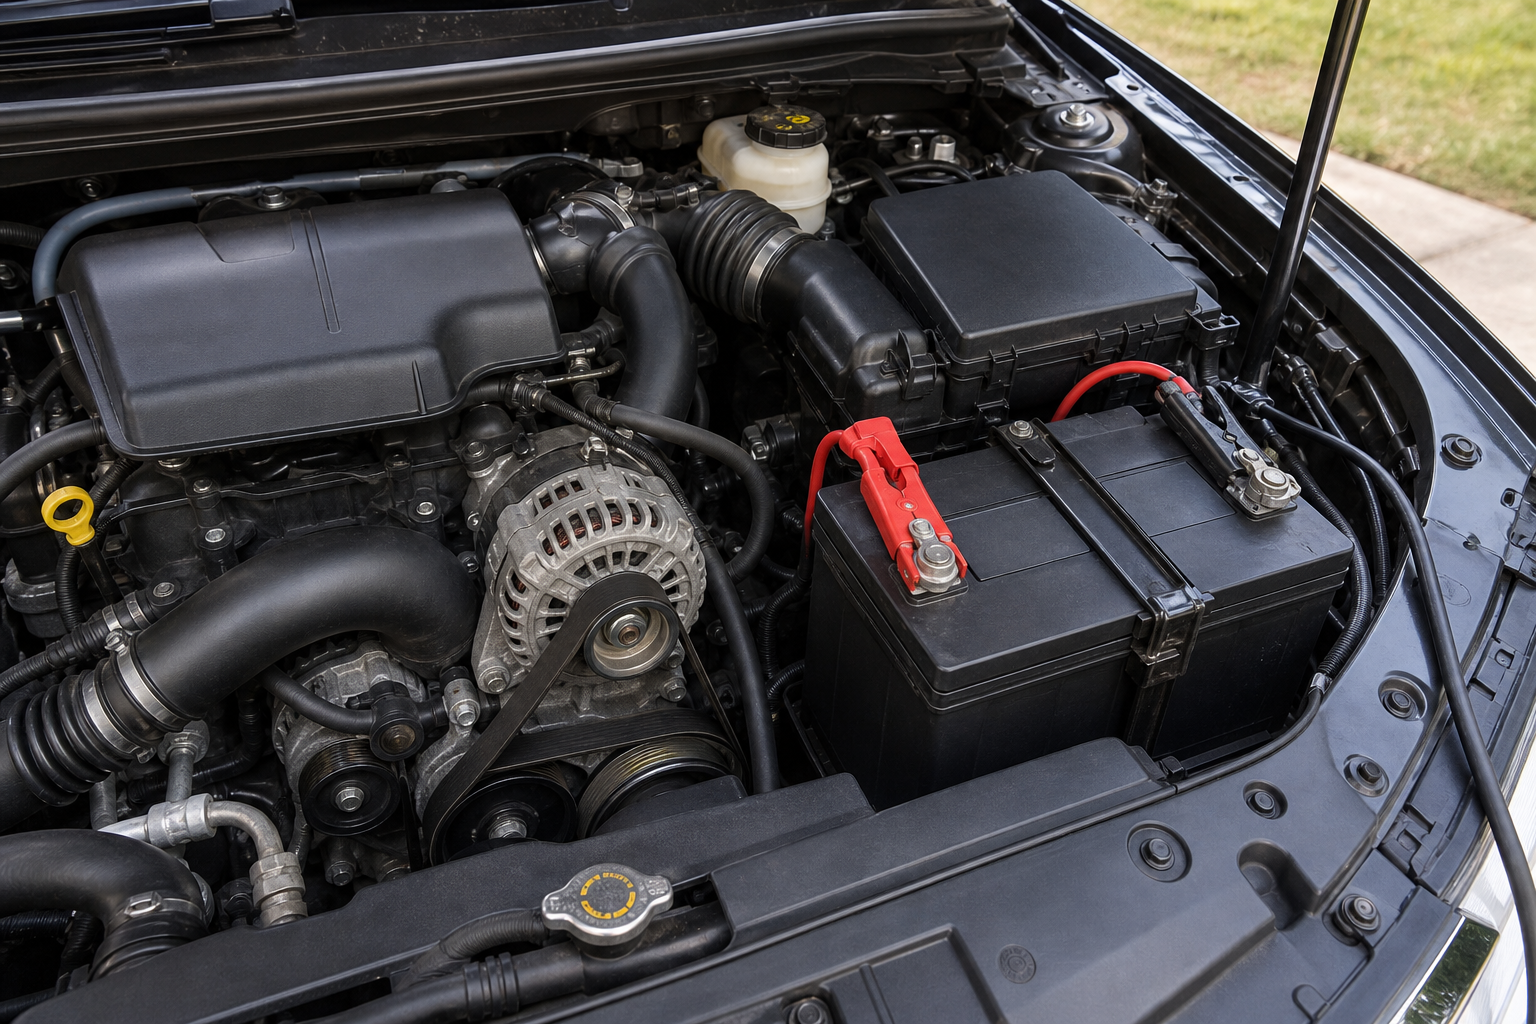
\includegraphics[width=0.58\linewidth]{images/book3/ai/b3-06-car-battery-engine-bay.png}

{\small Bajo el capó: la batería de \qty{12}{V}, sus cables gruesos y el alternador --- la red de corriente continua del problema de fin de semana, con centenares de \omterm{def:b1:dc-circuits:current}{amperios} en el arranque.}
\end{omfigure}

\section{Problema: la instalación eléctrica de un coche}

\begin{problem}[{Problema de fin de semana --- una batería, un motor de
arranque, dos faros, un alternador y unos metros de cobre: quién se lleva
la corriente, quién la paga y por qué bajan las luces al arrancar}]
\label{pb:b1:dc-circuits:1}
La batería es una fuente real de fem $E = \qty{12.6}{V}$ y \omterm{def:b1:dc-circuits:sources}{resistencia
interna} $r = \qty{10}{m\ohm}$. Cobre: $\rho = \qty{1.7e-8}{\ohm.m}$.

\medskip
\noindent\textbf{Parte I --- La batería sola.}
\begin{enumerate}
  \item Dibújese el modelo de Thévenin y escríbase $u(i)$ en el \omterm{thm:b1:dc-circuits:kirchhoff}{convenio
        generador}.
  \item Dense la \omterm{def:b1:dc-circuits:voltage}{tensión} en circuito abierto y la corriente de
        cortocircuito. ¿Por qué una llave caída no debe puentear nunca los
        bornes?
  \item Escríbase el modelo de Norton de esa misma batería.
  \item La batería alimenta un \omterm{def:b1:dc-circuits:resistor}{resistor} $R$: exprésense la corriente, la
        \omterm{def:b1:dc-circuits:voltage}{tensión} en bornes, la potencia $P_R$ entregada y la potencia
        perdida en $r$.
  \item Muéstrese que $P_R$ es máxima para $R = r$ y calcúlese ese
        máximo. ¿Cuál es entonces el rendimiento?
  \item Un técnico mide $u = \qty{12.48}{V}$ a \qty{12}{A} y
        $u = \qty{11.40}{V}$ a \qty{120}{A}. Compruébese que ambos puntos
        caen sobre el modelo y explíquese cómo una serie de puntos así da
        $E$ y $r$ mediante un ajuste por una recta.
  \item La batería almacena \qty{60}{A.h}. ¿Cuánto tiempo podría
        alimentar los dos faros de \qty{55}{W} sola (tómese \qty{12}{V})?
        ¿Cuánta energía es eso en julios?
\end{enumerate}

\medskip
\noindent\textbf{Parte II --- Arrancar con las luces encendidas.}
El motor de arranque es un \omterm{def:b1:dc-circuits:resistor}{resistor} $R_s = \qty{80}{m\ohm}$; cada faro es
de \qty{55}{W} a \qty{12.0}{V} y se trata como un \omterm{def:b1:dc-circuits:resistor}{resistor}.
\begin{enumerate}[resume]
  \item Calcúlense la resistencia de un faro y la de los dos en paralelo.
  \item Motor de arranque solo: corriente, \omterm{def:b1:dc-circuits:voltage}{tensión} en bornes, potencia en
        el motor de arranque y potencia perdida en la batería.
  \item Motor de arranque y los dos faros a la vez: resistencia de carga
        equivalente, corriente total y \omterm{def:b1:dc-circuits:voltage}{tensión} en bornes.
  \item Úsese el \omterm{prop:b1:dc-circuits:dividers}{divisor de corriente} para hallar la corriente del motor
        de arranque y la de los faros.
  \item Calcúlese la potencia que recibe ahora cada faro y compárese con
        su valor nominal: ¿en qué fracción se atenúan las luces?
  \item Explíquese en dos frases, con la \omterm{thm:b1:dc-circuits:kirchhoff}{ley de las mallas}, por qué las
        luces se atenúan precisamente porque el motor de arranque consume
        una corriente grande.
  \item ¿Ayudaría a las luces poner cables de batería más gruesos?
        Justifíquese de forma cualitativa por ahora (la Parte IV lo
        cuantifica).
\end{enumerate}

\medskip
\noindent\textbf{Parte III --- Motor en marcha: el alternador.}
El alternador es una segunda fuente real, $E_a = \qty{14.2}{V}$,
$r_a = \qty{50}{m\ohm}$, en paralelo con la batería; el motor de arranque
está parado y los dos faros encendidos.
\begin{enumerate}[resume]
  \item Dibújese el circuito: dos fuentes reales y la carga de los faros
        en paralelo entre los dos mismos nudos.
  \item Aplíquese el \omterm{prop:b1:dc-circuits:millman}{teorema de Millman} para hallar la \omterm{def:b1:dc-circuits:voltage}{tensión} común en
        bornes.
  \item Dedúzcanse la corriente del alternador, la de la batería (¡con su
        signo!) y la de los faros; compruébese la \omterm{thm:b1:dc-circuits:kirchhoff}{ley de los nudos}.
  \item ¿Se carga o se descarga la batería? ¿Qué potencia recibe y qué
        potencia suministra el alternador?
  \item Recupérese la \omterm{def:b1:dc-circuits:voltage}{tensión} en bornes por superposición (cada fuente
        sola, con la otra sustituida por su \omterm{def:b1:dc-circuits:sources}{resistencia interna}) y
        compruébese.
\end{enumerate}

\medskip
\noindent\textbf{Parte IV --- Sensores y cables.}
\begin{enumerate}[resume]
  \item El sensor de refrigerante es un termistor cuya resistencia baja de
        \qty{2.0}{k\ohm} a \qty{20}{\degreeCelsius} hasta \qty{300}{\ohm} a
        \qty{90}{\degreeCelsius}; es el \omterm{def:b1:dc-circuits:resistor}{resistor} inferior de un divisor
        alimentado a \qty{5.0}{V}, siendo $R_0$ el superior. Exprésese la
        \omterm{def:b1:dc-circuits:voltage}{tensión} de salida y calcúlese a ambas temperaturas para
        $R_0 = \qty{775}{\ohm}$.
  \item Muéstrese que la excursión de salida entre las dos temperaturas es
        máxima cuando $R_0$ es la media geométrica de los dos valores del
        sensor, y compruébese el valor anterior.
  \item El mismo sensor se monta en un \omterm{prop:b1:dc-circuits:wheatstone}{puente de Wheatstone} con otros tres
        \omterm{def:b1:dc-circuits:resistor}{resistores} de \qty{775}{\ohm}: escríbase la salida del puente y
        dígase a qué temperatura está equilibrado.
  \item El cable del motor de arranque mide \qty{1.5}{m} en cada sentido.
        Calcúlense la resistencia de un conductor de sección
        \qty{16}{mm^2}, la caída de \omterm{def:b1:dc-circuits:voltage}{tensión} total a \qty{140}{A} y la
        potencia disipada en los cables.
  \item Lo mismo con cable de \qty{4}{mm^2}: ¿por qué es tan grueso el
        cable del motor de arranque?
  \item Resúmase: dese la \omterm{def:b1:dc-circuits:voltage}{tensión} en bornes durante el arranque, la
        fracción de potencia que llega al motor de arranque y la única ley
        que explica la atenuación de las luces.
\end{enumerate}
\end{problem}
